%% vim:tw=66:spell:wrap:ft=tex:
\ifx \printpresenthandout \undefined
	\ifx \printpresentarticle \undefined
		% no handout and no article
		\documentclass{beamer}
	\else
		% print article
		\documentclass[11pt]{article}
		\usepackage{beamerarticle}
	\fi
\else
	% handout
	\documentclass[handout]{beamer}
\fi
% Preamble
%\usepackage[small,sf,bf]{titlesec}
\PassOptionsToPackage{table,x11names,dvipsnames,rgb}{xcolor}

\usepackage[utf8]{inputenc}
\usepackage[british]{babel}

\usepackage{xstring}

\usepackage{tikz}
\usetikzlibrary{arrows,shapes,automata,positioning,trees,shadows,mindmap,decorations}
%% From <http://tex.stackexchange.com/questions/137357/how-to-draw-an-arrow-with-two-colors>
%% <http://tex.stackexchange.com/a/137438>
\usetikzlibrary{fadings,decorations.pathmorphing}

\makeatletter
\newif\iftikz@shading@path

\tikzset{
    % There are three circumstances in which the fading sep is needed:
    % 1. Arrows which do not update the bounding box (which is most of them).
    % 2. Line caps/joins and mitres that extend outside the natural bounding 
    %    box of the path (these are not calculated by PGF).
    % 3. Other reasons that haven't been anticipated.
    shading xsep/.store in=\tikz@pathshadingxsep,
    shading ysep/.store in=\tikz@pathshadingysep,
    shading sep/.style={shading xsep=#1, shading ysep=#1},
    shading sep=0.0cm,
}

\def\tikz@shadepath#1{% 
    % \tikz@addmode installs the `modes' (e.g., fill, draw, shade) 
    % to be applied to the path. It isn't usualy for doing more
    % changes to the path's construction.
    \iftikz@shading@path%
    \else%
        \tikz@shading@pathtrue%
        % Get the current path.
        \pgfgetpath\tikz@currentshadingpath%
        % Get the shading sep without setting any other keys.
        \begingroup%
            \pgfsys@beginscope% <- may not be necessary
            \tikzset{#1}%
            \xdef\tikz@tmp{\noexpand\def\noexpand\tikz@pathshadingxsep{\tikz@pathshadingxsep}%
                \noexpand\def\noexpand\tikz@pathshadingysep{\tikz@pathshadingysep}}%
            \pgfsys@endscope%
        \endgroup
        \tikz@tmp%
        % Get the boudning box of the current path size including the shading sep
        \pgfextract@process\pgf@shadingpath@southwest{\pgfpointadd{\pgfqpoint{\pgf@pathminx}{\pgf@pathminy}}%
            {\pgfpoint{-\tikz@pathshadingxsep}{-\tikz@pathshadingysep}}}%%
        \pgfextract@process\pgf@shadingpath@northeast{\pgfpointadd{\pgfqpoint{\pgf@pathmaxx}{\pgf@pathmaxy}}%
            {\pgfpoint{\tikz@pathshadingxsep}{\tikz@pathshadingysep}}}%
        % Clear the path
        \pgfsetpath\pgfutil@empty%                          
        % Save the current drawing mode and options.
        \let\tikz@options@saved=\tikz@options%
        \let\tikz@mode@saved=\tikz@mode%
        \let\tikz@options=\pgfutil@empty%
        \let\tikz@mode=\pgfutil@empty%
        % \tikz@options are processed later on.
        \tikz@addoption{%
            \pgfinterruptpath%
            \pgfinterruptpicture%
                \begin{tikzfadingfrompicture}[name=.]
                \pgfscope%
                    \tikzset{shade path/.style=}% Make absolutely sure shade path is not inherited.
                    \path \pgfextra{%
                        % Set the softpath. Any transformations,draw=none} in #1 will have no effect.
                        % This will *not* update the bounding box...
                        \pgfsetpath\tikz@currentshadingpath%
                        % ...so it is done manually.
                        \pgf@shadingpath@southwest
                        \expandafter\pgf@protocolsizes{\the\pgf@x}{\the\pgf@y}%
                        \pgf@shadingpath@northeast%
                        \expandafter\pgf@protocolsizes{\the\pgf@x}{\the\pgf@y}%
                        % Install the drawing modes and options.
                        \let\tikz@options=\tikz@options@saved%
                        \let\tikz@mode=\tikz@mode@saved%
                    };
                    % Now get the bounding box of the picture.
                    \xdef\pgf@shadingboundingbox@southwest{\noexpand\pgfqpoint{\the\pgf@picminx}{\the\pgf@picminy}}%
                    \xdef\pgf@shadingboundingbox@northeast{\noexpand\pgfqpoint{\the\pgf@picmaxx}{\the\pgf@picmaxy}}%
                    \endpgfscope
                \end{tikzfadingfrompicture}%
            \endpgfinterruptpicture%
            \endpgfinterruptpath%
            % Install a rectangle that covers the shaded/faded path picture.
            \pgftransformreset%
            \pgfpathrectanglecorners{\pgf@shadingboundingbox@southwest}{\pgf@shadingboundingbox@northeast}%
            %
            % Reset all modes.
            \let\tikz@path@picture=\pgfutil@empty%
            \tikz@mode@fillfalse%
            \tikz@mode@drawfalse%
            \tikz@mode@tipsfalse%
            \tikz@mode@doublefalse%
            \tikz@mode@clipfalse%
            \tikz@mode@boundaryfalse%
            \tikz@mode@fade@pathfalse%
            \tikz@mode@fade@scopefalse%
            % Now install shading options.
            \tikzset{#1}%
            \tikz@mode%
            % Make the fading happen.
            \def\tikz@path@fading{.}%
            \tikz@mode@fade@pathtrue%
            \tikz@fade@adjustfalse%
            % Shift the fading to the mid point of the rectangle
            \pgfpointscale{0.5}{\pgfpointadd{\pgf@shadingboundingbox@southwest}{\pgf@shadingboundingbox@northeast}}%
            \edef\tikz@fade@transform{shift={(\the\pgf@x,\the\pgf@y)}}%
            \pgfsetfading{\tikz@path@fading}{\tikz@do@fade@transform}%
            \tikz@mode@fade@pathfalse%              
        }%
    \fi%
}
\tikzset{
    shade path/.code={%
        \tikz@addmode{\tikz@shadepath{#1}}%
    }
}

% requires tikz
\usepackage{colortbl}

\usepackage{float}
\usepackage{graphicx}
\usepackage[normalem]{ulem}

%% use as
%%     \vertcenterimage{\includegraphics{*}}
\newcommand{\vertcenterimage}[1]{\raisebox{-.5\height}{#1}}

%% use as
%%     \flipbox{\includegraphics{*}}
\newcommand{\flipbox}[1]{\scalebox{1}[-1]{#1}}

\usepackage{amsmath}
\usepackage{amsfonts}
\usepackage{bm} % bold mathematics (\bm command)

% set-builder notation using \Set{ ... | ... }
\usepackage{braket}

\usepackage{mathtools}
\usepackage{breqn}

%% make everything in the box bold; both the text and mathematics: using
%% \boldmath from `bm` package
\newcommand{\be}{\bfseries\boldmath}

\usepackage{pifont}% http://ctan.org/pkg/pifont
\newcommand{\cmark}{\ding{51}}%
\newcommand{\xmark}{\ding{55}}%

\newcommand{\todo}[1]{%
	\textcolor{red}{TODO: #1}%
}
\newcommand{\todofig}[1]{%
	\textcolor{red}{TODO figure: \nolinkurl{#1}}%
}


\usepackage{hyperref}
\hypersetup{%
	pdfauthor={Zakariyya Mughal},%
	pdfpagemode={None},%
	pdfpagelayout={SinglePage}%
}


\usetheme{Ilmenau}
\usecolortheme{beaver}
\usepackage{ifxetex}

\ifxetex
	% set font to Tahoma
	\usefonttheme{professionalfonts} % using non standard fonts for beamer
	\usefonttheme{serif} % default family is serif
	\usepackage{fontspec}
	\setmainfont{Tahoma}
\else
	\usepackage[T1]{fontenc}
\fi

\definecolor{CBLRed}{RGB}{205,0,0}

\colorlet{langC}{blue!40}
\colorlet{langM}{orange!20}
\colorlet{data}{grey!10}

% Title on title slide
\setbeamerfont{title}{size = \Large}
\setbeamercolor{title}{fg = black, bg = white}

\setbeamercolor{frametitle}{fg=white,bg=CBLRed}
\setbeamercolor{section in head/foot}{fg=white,bg=CBLRed}
\setbeamercolor{subsection in head/foot}{fg=white,bg=CBLRed}
\setbeamercolor{author in head/foot}{fg=white,bg=CBLRed}
\setbeamertemplate{headline}{}
\beamertemplatenavigationsymbolsempty

\logo{}
\def\insertlogo
{%
	\color{gray}
	\begin{tabular*}{\paperwidth}{p{0.01\paperwidth}p{0.84\paperwidth}p{0.15\paperwidth}}
		&
		\parbox[c][][c]{\textwidth}{\raggedright
			\vertcenterimage{
\includegraphics[width=\textwidth]{gfx/cbl-footer.png}}
		}
		&
		\parbox[c][][c]{\textwidth}{%\raggedleft
			{\large\insertframenumber} %/\inserttotalframenumber
		}
	\end{tabular*}
 }

%\usefonttheme[onlymath]{serif}
\ifx \printpresentarticle \undefined
	\setbeamertemplate{frametitle}[default][center]
	\setbeamertemplate{footline}{}
	%\setbeamertemplate{footline}[frame number]

	%% Change beamer bullets to circles rather than the ball default
	\setbeamertemplate{itemize items}[circle]
	\setbeamertemplate{enumerate items}[circle]
\fi


\usepackage{textcomp}
\usepackage{fancyvrb}
\usepackage{changepage}
\usepackage{multicol}
\usepackage{wasysym}
\usepackage{listings}

\lstset{%basicstyle=\small\ttfamily,
%numbers=left,
%escapeinside=||
}
\newenvironment{indented}{\begin{adjustwidth}{1.5em}{}}{\end{adjustwidth}}

% http://tex.stackexchange.com/questions/12550/changing-default-width-of-blocks-in-beamer/12551#12551
\newenvironment<>{varblock}[2][.9\textwidth]{%
  \setlength{\textwidth}{#1}
  \begin{actionenv}#3%
    \def\insertblocktitle{#2}%
    \par%
    \usebeamertemplate{block begin}}
  {\par%
    \usebeamertemplate{block end}%
  \end{actionenv}}

\ifx \printpresentnote \undefined
% no notes
\else
\setbeameroption{show only notes}
\fi

%% use as
%%     \af{ number of overlay }{ slide label }
%% e.g.,
%%     \af{2}{intro-slide}
\newcommand{\af}[2]{\againframe<#1|handout:0>[noframenumbering]{#2}}


%% TOC at beginning of sections/subsections
\ifx \printpresenthandout \undefined
	% no handout
	\AtBeginSubsection[]
	{
		\begin{frame}[noframenumbering]\frametitle{Table of contents}
			\begin{multicols}{2}
				\tableofcontents[
					currentsection,
					hideothersubsections,
					sectionstyle=show/shaded,
					subsectionstyle=show/shaded/hide,
				]
			\end{multicols}
	  \end{frame}
	}
\else
	\AtBeginSection[]
	{
		\begin{frame}[noframenumbering]\frametitle{Table of contents}
			\begin{multicols}{2}
				\tableofcontents[
					currentsection,
					currentsubsection,
					hideothersubsections,
					sectionstyle=show/shaded,
					subsectionstyle=show/show/hide,
				]
			\end{multicols}
	  \end{frame}
	}
\fi

%% TikZ arrows
%% From <https://tex.stackexchange.com/questions/61507/drawing-arrows-in-beamer>
\tikzset{
    myarrow/.style={
        draw,
        fill=orange,
        single arrow,
        minimum height=3.5ex,
        single arrow head extend=1ex
    }
}
\newcommand{\arrowup}{%
\tikz [baseline=-0.5ex]{\node [myarrow,rotate=90] {};}
}
\newcommand{\arrowdown}{%
\tikz [baseline=-1ex]{\node [myarrow,rotate=-90] {};}
}
\newcommand{\arrowright}{%
\tikz [baseline=-0.5ex]{\node [myarrow,rotate=0] {};}
}
\newcommand{\arrowleft}{%
\tikz [baseline=-0.5ex]{\node [myarrow,rotate=180] {};}
}


\definecolor{quotemark}{gray}{0.7}
\newenvironment{fancyquote}%
	{%
	    \vspace{1em}%
	    \singlespacing
	    \noindent%
		 \begin{picture}(0,0)%
		 \put(-15,-0){\makebox(0,0){\scalebox{3}{\textcolor{quotemark}{``}}}}%
		 \end{picture}%
	\footnotesize\upshape%
	}%
	{%
	 \par%
	 \makebox[0pt][l]{%
	 \hspace{\linewidth}%
	 \begin{picture}(0,0)(0,0)%
	 \put(15,20){\makebox(0,0){%
	 \scalebox{3}{\color{quotemark}''}}}%
	 \end{picture}}%
	   \vspace{-2.5em}%
	}%


\usepackage{diagbox}

\usepackage{fontawesome}
\colorlet{tbackground}{blue!80}
\colorlet{tobjectives}{red!80}
\colorlet{tmetrics}{green!120}
\ifx \tcolor \undefined
	% no color
	\newcommand{\tbackground}[1]{#1}
	\newcommand{\tobjectives}[1]{#1}
	\newcommand{\tmetrics}[1]{#1}
\else
	\newcommand{\tbackground}[1]{\textcolor{tbackground}{#1}}
	\newcommand{\tobjectives}[1]{\textcolor{tobjectives}{#1}}
	\newcommand{\tmetrics}[1]{\textcolor{tmetrics}{#1}}
\fi

%%% From
%% <http://tex.stackexchange.com/questions/118939/add-watermark-that-overlays-the-images>
%% <http://tex.stackexchange.com/questions/132582/transparent-foreground-watermark>
\usepackage[printwatermark]{xwatermark}
%% Water mark in the background
%\newwatermark[allpages,color=red!10,angle=45,scale=3,xpos=0,ypos=0]{DRAFT}

\newsavebox\mydraftbox
\savebox\mydraftbox{\tikz[color=red!50,opacity=0.3]\node{DRAFT};}
\newwatermark*[allpages,angle=45,scale=6,xpos=-20,ypos=15]{\usebox\mydraftbox}


 \edef\defaultpgflinewidth{\the\pgflinewidth}

%% PGF change color decoration for path
\makeatletter
\pgfkeys{/pgf/decoration/.cd, start color/.store in =\startcolor, end color/.store in   =\endcolor, visibility/.estore in =\decorateopacity}
\pgfdeclaredecoration{color change}{initial}{
 \state{initial}[width=0pt, next state=line, persistent precomputation={%
   \pgfmathdivide{50}{\pgfdecoratedpathlength}%
   \let\increment=\pgfmathresult%
   \let\dop=\decorateopacity%
   \def\x{0}%
 }]{}
 \state{line}[width=.5pt,   persistent postcomputation={%
     \pgfmathadd@{\x}{\increment}%
     \let\x=\pgfmathresult%
   }]{%
   %\pgfsetlinewidth{1\defaultpgflinewidth}%
   \pgfsetarrows{-}%
   \pgfpathmoveto{\pgfpointorigin}%
   \pgfpathlineto{\pgfqpoint{.75pt}{0pt}}%
   \pgfsetstrokeopacity{\decorateopacity}%
   \pgfsetstrokecolor{\endcolor!\x!\startcolor}%
   \pgfusepath{stroke}%
 }
 \state{final}{%
   \pgfsetlinewidth{\defaultpgflinewidth}%
   \pgfpathmoveto{\pgfpointorigin}%
   \color{\endcolor!\x!\startcolor}%
   \pgfusepath{stroke}%
 }}
\makeatother

% Styles
\tikzstyle{function} = [draw,fill=blue!60,shape=rectangle, text centered,text=white, text width=3cm, minimum size=2.5cm]
\tikzstyle{data}     = [draw,fill=orange,shape=ellipse, text centered,text=white, text width=2.5cm, minimum size=2.5cm]
\tikzstyle{d2f}  = [draw, line width = 2pt,
      decoration = {color change, start color=blue, end color=orange},
      decorate]
\tikzstyle{f2d}  = [draw, line width = 2pt,
      decoration = {color change, start color=orange, end color=blue},
      decorate]


\begin{document}
% meta needs to be in \begin{document} so that tabular works
\title[]{Converting a Neuron Morphology Reconstruction System: Open Science Design and Implementation}
\author[]{Zakariyya Mughal}
\institute[]{Computational Biomedicine Lab\\University of Houston}
\date{2015 Nov 30}

%% transitions are made transparent rather than hidden
\setbeamercovered{transparent}
\newcommand{\SegGroundTotal}{\ensuremath{S_{\mathrm{G,T}}}}
\newcommand{\SegAutomaticTotal}{\ensuremath{S_{\mathrm{A,T}}}}
\newcommand{\SegAutomaticCorrect}{\ensuremath{S_{\mathrm{A,C}}}}
\newcommand{\SegAutomaticMissing}{\ensuremath{S_{\mathrm{A,miss}}}}
\newcommand{\SegAutomaticExtra}{\ensuremath{S_{\mathrm{A,extra}}}}

% TODO Notation and stylistic conventions


\newglossaryentry{fn}{%
	name={\ensuremath{F_n}},%
	sort=fn,%
	description={Empirical (sample) distribution function}}

\newglossaryentry{fncon}{%
	name={\ensuremath{F^{n^\ast}}},%
	sort=fnc,%
	description={$n$-fold convolution of the distribution function/distribution $F$}}


\makeglossaries

%  - Title slide.%{{{
\frame{\titlepage}
%}}}

\ifx \tcolor \undefined
\else
	The following text is color-coded based on what kind of
	information it provides the audience:
	\tbackground{background information},
	\tobjectives{objectives},
	\tmetrics{metrics for completion of objectives}.
\fi

\ifx \printpresentarticle \undefined \else
	\tableofcontents
\fi

\section{Background}
\subsection{Neuron reconstruction}
\begin{frame}\frametitle{\subsecname}
	\centering
	\begin{tabular}{c}
	\vertcenterimage{\flipbox{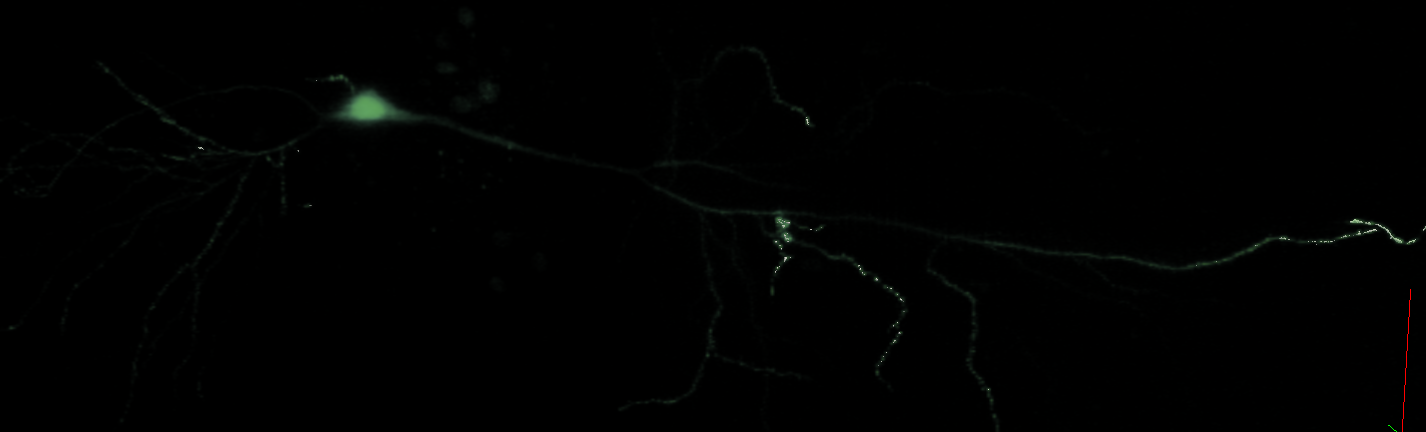
\includegraphics[width=0.8\textwidth]{gfx/present/neuron-vol}}} \\\\
	\arrowdown \\\\
	\vertcenterimage{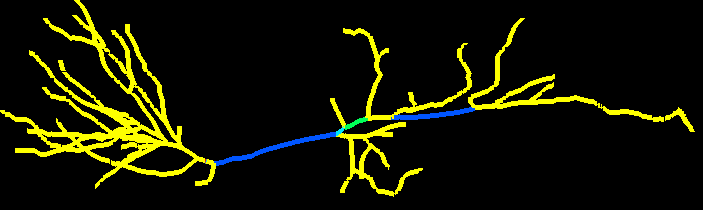
\includegraphics[width=0.8\textwidth]{gfx/present/neuron-trace}}
	\end{tabular}
	\note{%
		Data
		[\tbackground
			{%
				what is neuron reconstruction; data acquisition; image analysis; why
				automate (i.e., why automated neuron
				tracing research is important);
				mention ORION
			}
		]
	}
	\note{
		% TODO more notes
		\begin{itemize}
		\item
		  confocal and two-photon microscopy
		\item
		  fluorescent proteins on a single neuron
		\item
		  sampled in 3D
		\item
		  problems with manual tracing

		  \begin{itemize}
		  \item
		    slow: can take up to 24 hours of work by domain expert on a single
		    neuron
		  \item
		    difficult in 3D
		  \end{itemize}
		\item
		  problems in general

		  \begin{itemize}
		  \item
		    faint intensity
		  \item
		    lots of noise
		  \end{itemize}
		\end{itemize}
	}
\end{frame}

\subsection{Open science}
\begin{frame}\frametitle{\subsecname}
\centering
\begin{tabular}{p{0.6\textwidth}c}
	\begin{minipage}{\linewidth}
	\begin{quote}
		\begin{fancyquote}
		Open science is the idea that scientific knowledge of all kinds
		should be openly shared as early as is practical in the discovery
		process.
		\end{fancyquote}
		--- \qauthor{Michael Nielsen}
	\end{quote}
	\end{minipage}
	&
	\vertcenterimage{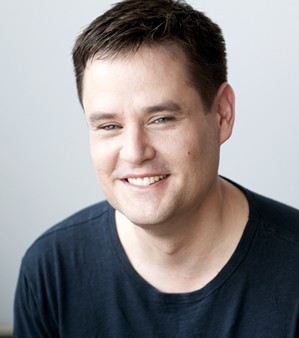
\includegraphics[height=0.3\textheight]{gfx/present/michael-nielsen}}
\end{tabular}
	\note{
		% TODO more notes
		Scientific knowledge
		\begin{itemize}
		\item
		  problem definitions
		\item
		  ideas
		\item
		  code
		\item
		  data
		\item
		  methodology
		\item
		  journal articles
		\end{itemize}
	}
	\note{
		% TODO more notes
		[\tbackground
			{%
			what it means to be an open-science project (i.e., open release of all
			research artifacts as early as possible)
			}
		]
	}
\end{frame}

\subsection{BigNeuron}
\begin{frame}\frametitle{\subsecname}
	\centering
	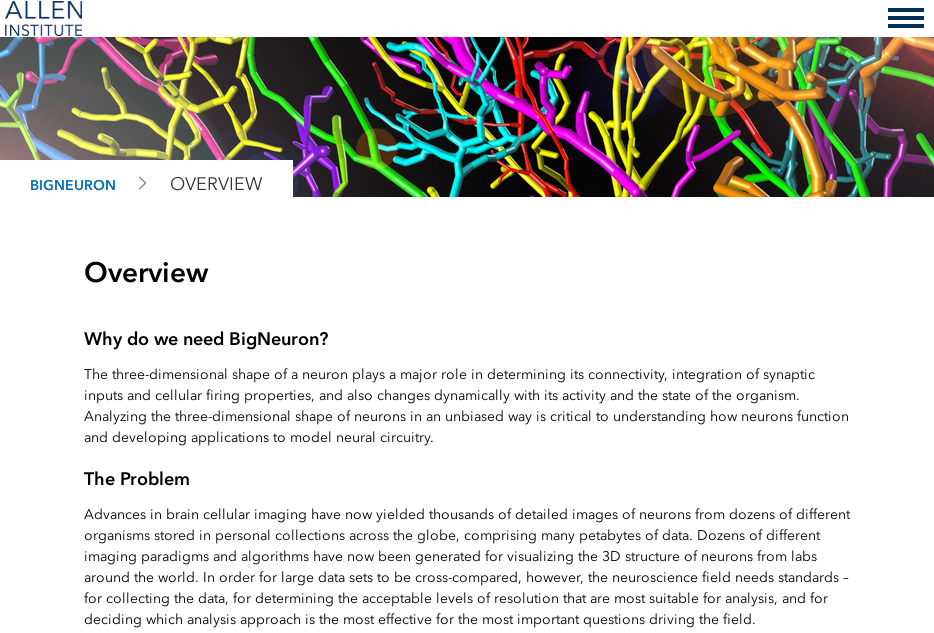
\includegraphics[height=0.6\textheight]{gfx/bigneuron-website}
	\note{
		% TODO more notes
		[\tbackground
			{%
				goal of BigNeuron and purpose of participation in
				BigNeuron and how each algorithm must be released under
				open-science
			}
		]
	}
	\note{
		% TODO more notes
		\begin{itemize}
		\item
		  Continuing where the DIADEM Challenge left off
		\item
		  Comparing algorithms across large datasets
		\item
		  Stitching multiple neuron reconstructions together
		\end{itemize}
	}
\end{frame}

\section{Problem}
%  - Problem Statement - Goals, objectives, aims. May also include challenges.
%        IMPORTANT: State your specific aims clearly - what you plan to achieve and how
%        you plan to achieve it. Let your contributions to the field of Computer Science
%        be clear.
\begin{frame}\frametitle{\secname}
	\Huge
	\renewcommand{\arraystretch}{1.5}% Spread rows out...
	\begin{tabular}{m{5em}m{1em}m{4em}m{1em}}
		BigNeuron & + & \vertcenterimage{
\includegraphics[height=2em]{gfx/present/mathworks-logo}} & \textcolor{red}{\xmark} \\[1em]
		BigNeuron & + & C/C++ & \textcolor{green}{\cmark}
	\end{tabular}
	\note{
		% TODO more notes
		[\tbackground{explain how the ORION code exists in MATLAB form but is difficult to
		integrate into BigNeuron}; explain challenges in later slides]
	}
\end{frame}

\section{Goal}
%  - Motivation - short introduction to your research, pointers to applications, why the research is important.
\begin{frame}\frametitle{\secname}
	\centering
	\tobjectives{%
	The reimplementation of  a system
	%
		for \alert{neuron reconstruction}
	%
		that is distributed as an \alert{open-science} project
		and
	%
		compatible with the \alert{BigNeuron} project.
	%
	}
\end{frame}

\subsection{Objectives}
\begin{frame}\frametitle{\subsecname}
	\tobjectives{%
	% TODO choose icons for each objective to put in the slide
	% headers
	% - conversion : recycle? \faRecycle
	% - integration: gears? \faCogs
	% - testing: Erlenmeyer flask (for science)? \faFlask
	\begin{enumerate}[<+->]
		\setlength\itemsep{1em}
		\item convert the ORION algorithm: \faRefresh
			\begin{center}
				\gls{orionmat} $\rightarrow$ \gls{orionc};
			\end{center}
		\item integrate \gls{orionc} with Vaa3D; \faCogs{}
			and % "and" before last item
		\item create a test suite and ensure
			reproducible results. \faCheckSquareO % end of sentence

	\end{enumerate}
	}
\end{frame}

\section{Context}
%  - Related Work - a catchy name is “State of the Art”.
%        Literature review relevant to specific research. Your committee
%        members are expected to already have a general background in your field.
%        Concentrate on the details of your specific research area. It is preferable to
%        use more recent literature (except for some classical “old” ones). Also avoid
%        reviewing standard concepts that have been around for a long time.
\begin{frame}\frametitle{\secname}
	\tbackground{%
	\begin{itemize}
		\item Prior work in \alert{neuron reconstruction}
		\item Principles of \alert{open-science}
		\item An overview of \alert{BigNeuron}
	\end{itemize}
	}
\end{frame}

\subsection{Neuron reconstruction}
\begin{frame}\frametitle{\subsecname}
	\begin{multicols}{2}
	\begin{itemize}
		\item<1-> Golgi~staining --- Camillo~Golgi (1873)
		\item<2-> Improved by Ram\'on~y~Cajal (1887)
	\end{itemize}
	\columnbreak
	\begin{tikzpicture}[node distance=2cm]
		\node (img1)
			{{\includegraphics<1->[width=0.3\textwidth]{gfx/present/Golgi_Hippocampus.jpg}}};
		\node[below right of=img1] (img2)
			{{\includegraphics<2->[width=0.3\textwidth]{gfx/present/cajal-chick-cerebellum.jpg}}};
		%\pause
		%\node (img3) at (img2.south west) [yshift=1cm] {\includegraphics[height=3cm]{img3}};
	\end{tikzpicture}
	\end{multicols}
	\note{
		reticular theory vs. neuron doctrine

		[\tbackground{explain the problem of neuron reconstruction; history of
		neuron tracing; biological relevance and applications}]
	}
\end{frame}

\begin{frame}\frametitle{Digital neuron reconstruction}
	\begin{multicols}{2}
	\begin{itemize}
		\item<1-> The early days (late 1960s): digital acquisition
		\item<2-> Manual tracing (1980s -- late 1990s): NeuroLucida
		\item<3-> DIADEM (2009 -- 2010)
	\end{itemize}
	\columnbreak
	% TODO image of computer-microscope system
	\end{multicols}
	\note{
		% TODO
	}
\end{frame}

\subsubsection{DIADEM Challenge}
\begin{frame}\frametitle{\subsubsecname}
	% TODO
	\begin{center}
	\begin{tabular}{p{0.3\textwidth}p{0.3\textwidth}p{0.3\textwidth}}
	\be \begin{center}CF\end{center} & \be \begin{center}CA3\end{center} & \be \begin{center}NL1\end{center} \\
	\vertcenterimage{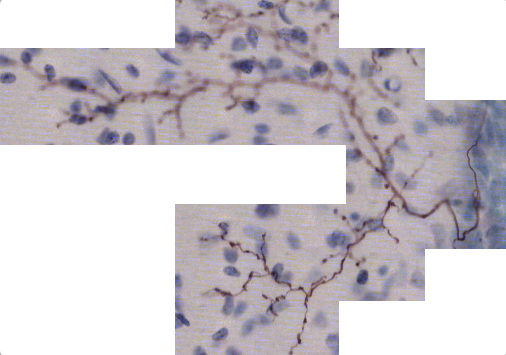
\includegraphics[width=0.3\textwidth]{gfx/vaa3D-DIADEM-1-CF_1-MIP.png}}
	& \vertcenterimage{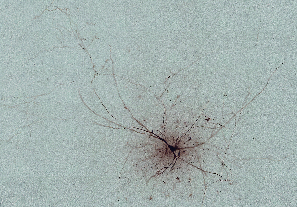
\includegraphics[width=0.3\textwidth]{gfx/vaa3D-DIADEM-2-HCA3-Section-1-MIP.png}}
	& \vertcenterimage{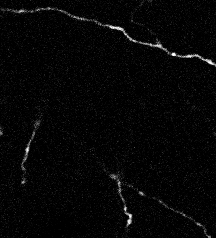
\includegraphics[width=0.2\textwidth]{gfx/vaa3D-DIADEM-3-NL1-01-MIP.png}} \\
	%
	\vertcenterimage{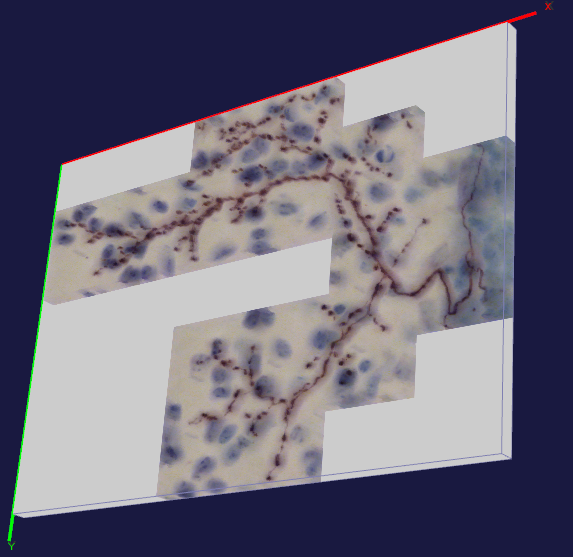
\includegraphics[width=0.2\textwidth]{gfx/vaa3D-DIADEM-1-CF_1-3D.png}}
	& \vertcenterimage{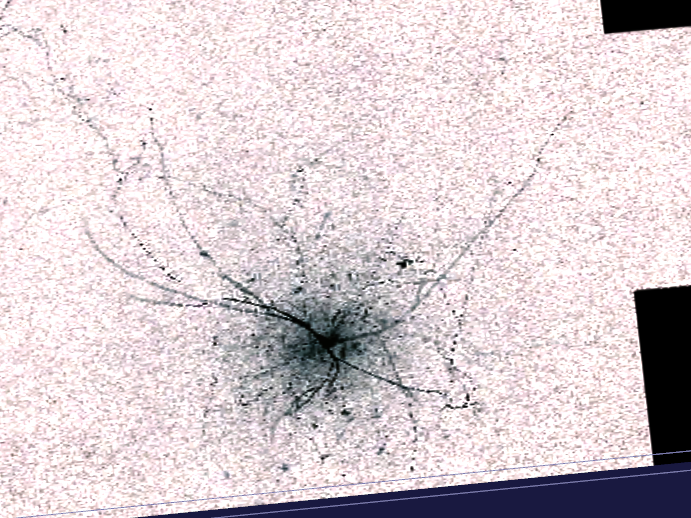
\includegraphics[width=0.2\textwidth]{gfx/DIADEM-dataset/x-selection-gray-dt2.png}}
	& \vertcenterimage{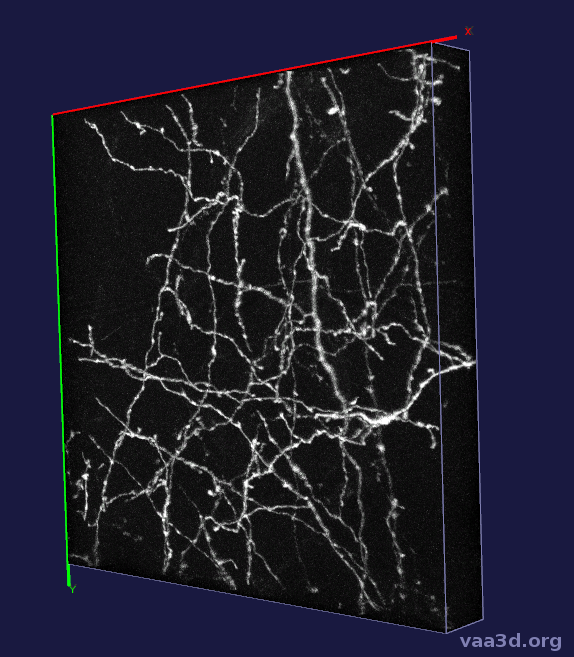
\includegraphics[width=0.2\textwidth]{gfx/vaa3D-DIADEM-3-NL1-01-3D.png}}
	\end{tabular}
	\end{center}
	\note{
		[\tbackground{explain DIADEM Challenge; data sets; outcomes}]
	}
\end{frame}

\begin{frame}\frametitle{\subsubsecname}
	% TODO
	\begin{center}
	\begin{tabular}{p{0.3\textwidth}p{0.3\textwidth}p{0.3\textwidth}}
	 \be \begin{center}NPF\end{center} & \be \begin{center}OP\end{center} & \be \begin{center}CL\end{center} \\
		\vertcenterimage{
\includegraphics[width=0.2\textwidth]{gfx/DIADEM-dataset/x-selection-default-dt4-im25.png}}
		& \vertcenterimage{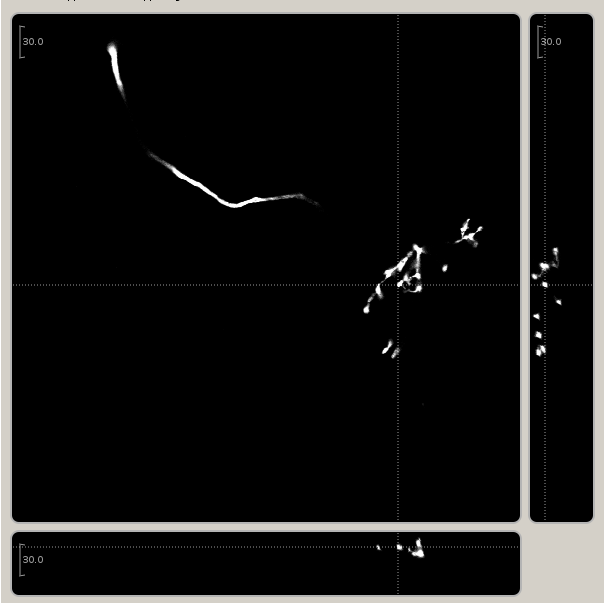
\includegraphics[width=0.2\textwidth]{gfx/DIADEM-dataset/2d-default-dt5-v2.png}}
		& \vertcenterimage{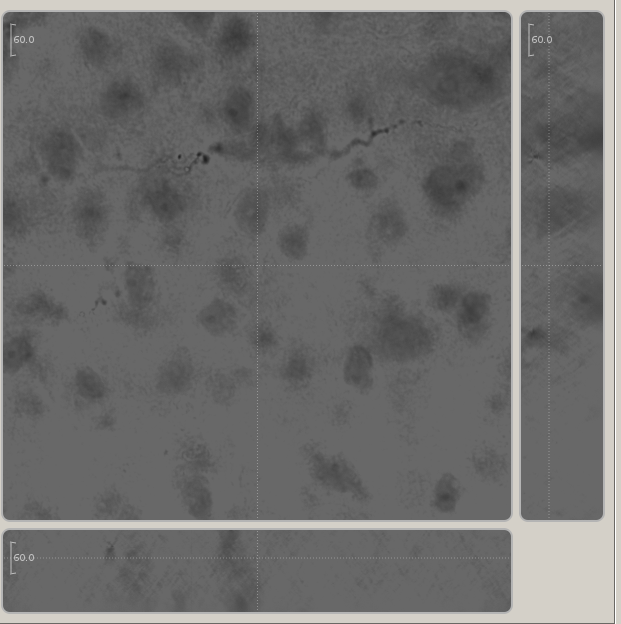
\includegraphics[width=0.2\textwidth]{gfx/DIADEM-dataset/2d-custom-dt6.png}} \\
		%
		\vertcenterimage{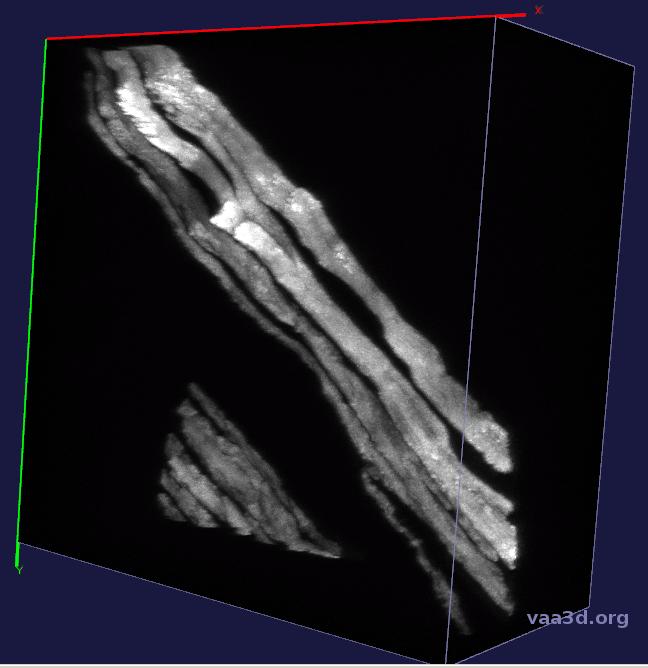
\includegraphics[width=0.2\textwidth]{gfx/DIADEM-dataset/MIP-default-dt4-im25.png}}
		& \vertcenterimage{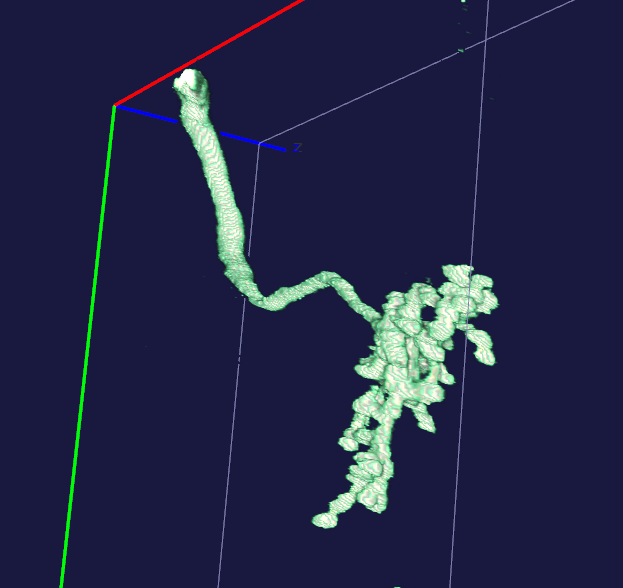
\includegraphics[width=0.2\textwidth]{gfx/DIADEM-dataset/alpha-default-dt5-v2.png}}
		& \vertcenterimage{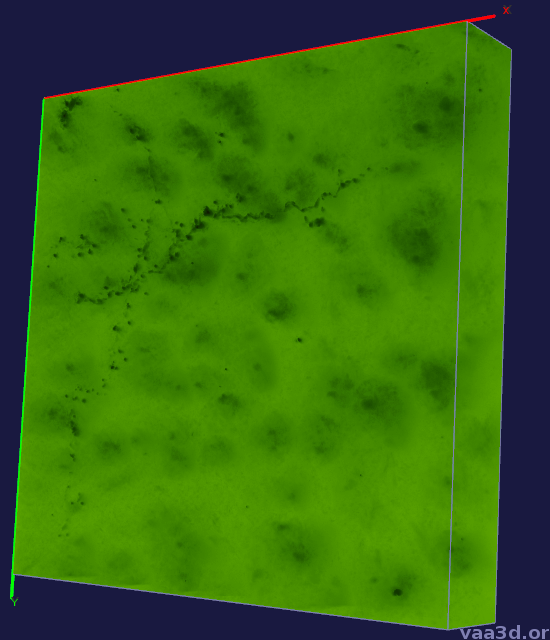
\includegraphics[width=0.2\textwidth]{gfx/DIADEM-dataset/mIP-custom-dt6-v2.png}}
	\end{tabular}
	\end{center}
	\note{
		[\tbackground{explain DIADEM Challenge; data sets; outcomes}]
	}
\end{frame}

%\subsubsection{Metrics}
%\begin{frame}\frametitle{\subsubsecname}
	%% TODO
	%\note{
	%[\tbackground{Create a table of metrics (e.g., precision, recall,
	%DIADEM metric, btmorph, NetMets) and explain how they work}]
	%}
%\end{frame}

%\subsubsection{Methods}
%\begin{frame}\frametitle{\subsubsecname}
	%% TODO
	%[\tbackground{Create a table of methods: what data they work with (2D/3D), modality,
	%metrics, what datasets they validated against}]
%\end{frame}

\subsection{Open science}
\begin{frame}\frametitle{\subsecname}
	\begin{itemize}
		\item Make research as public as much as possible
		\item Ensure that software/data can be run again
		\item Related: open access publishing, open data
	\end{itemize}
\end{frame}

\subsubsection{``Bermuda Principles''}
\begin{frame}\frametitle{\subsubsecname}
	Bermuda Principles (1996):
	\begin{itemize}
		\item data available in 24 hours of sequence assembly
		\item immediate publication of annotated sequences
		\item all data in the public domain
	\end{itemize}
	\note{
		\begin{itemize}
		\item
		  Human Genome Project: one of the earliest open research projects; 20 institutions from around the world; 13 years
		\item
		  arose after patent of breast cancer gene (BRCA2)
		\end{itemize}
	}
	\note{
	% TODO
	[\tbackground{explain ``Bermuda Principles'' from Human Genome Project
	(early large-scale open research project)}]
	}
\end{frame}

\subsubsection{Open science projects}
\begin{frame}\frametitle{\subsubsecname}
\centering
\begin{tabular}{cc}
	% Human Genome Project
	
\includegraphics[height=0.3\textheight]{gfx/present/HGP}
	&
	% OpenWorm
	
\includegraphics[height=0.3\textheight]{gfx/present/OpenWormLogo}
	\\
	% Galaxy Zoo
	
\includegraphics[height=0.3\textheight]{gfx/present/Galaxyzoo}
	&
	% Allen Brain Atlas
	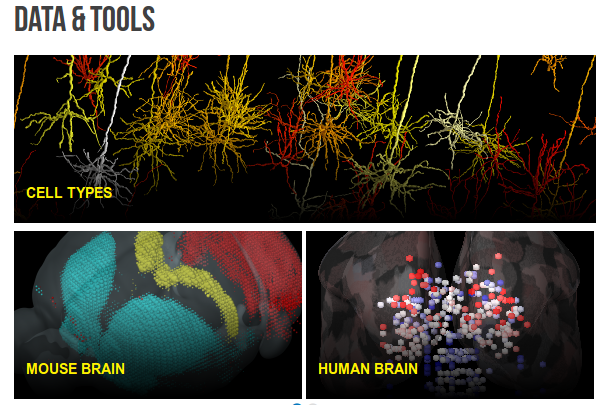
\includegraphics[height=0.3\textheight]{gfx/present/allen_brain_atlas_screenshot}
\end{tabular}
	\note{
		\begin{itemize}
		\item
		  Human Genome Project
		\item
		  OpenWorm: \emph{C. elegans} connectome modelling
		\item
		  GalaxyZoo: crowd-source classification of galaxies
		\item
		  Allen Brain Atlas: anatomical atlases of mouse and human brain
		\end{itemize}
	}
	% TODO
	\note{
	[\tbackground{showcase a few open science projects to show breadth}]
	}
\end{frame}

\begin{frame}\frametitle{Reproducibility for computational science}
	\begin{itemize}
	\item
	  Much of modern science is computational
	\item
	  SSI survey of researchers:

	  \begin{itemize}
	  \item
	    56\% code
	  \item
	    21\% of those: no training in software
	  \end{itemize}
	\item
	  RETRACTIONS
	\item
	  Unit tests not validation tests
	\item
	  Test many environments
	\end{itemize}
	\note{
		\begin{itemize}
		\item Note that the number is lowered since this include
			non-STEM fields. The numbers are as high as 85\% in STEM.
		\item
		  Give example of chemistry handedness mistake in protein structure
		  analysis.
		\item
		  Test step-by-step, not just look to see if the results look right
		\end{itemize}
	}
\end{frame}

\subsection{BigNeuron}
\begin{frame}\frametitle{\subsecname}
	\centering
	
\includegraphics[height=0.3\textheight]{gfx/present/alleninsitute12}
	\note{
	% TODO
	[\tbackground{explain what BigNeuron is; how it relates to this thesis;
		neuron stitching; bench testing}]
	}
\end{frame}

\subsubsection{Vaa3D}
\begin{frame}\frametitle{\subsubsecname}
	\centering
	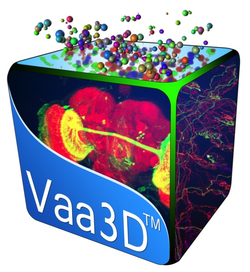
\includegraphics[height=0.5\textheight]{gfx/present/vaa3d-logo}
	\note{
		Standardising on Vaa3D image analysis tool
	}
	\note{
	% TODO
	[\tbackground{explain how Vaa3D has a plugin architecture and how it
	standardizes the BigNeuron project}]
	}
\end{frame}

\begin{frame}\frametitle{Vaa3D}
	\centering
	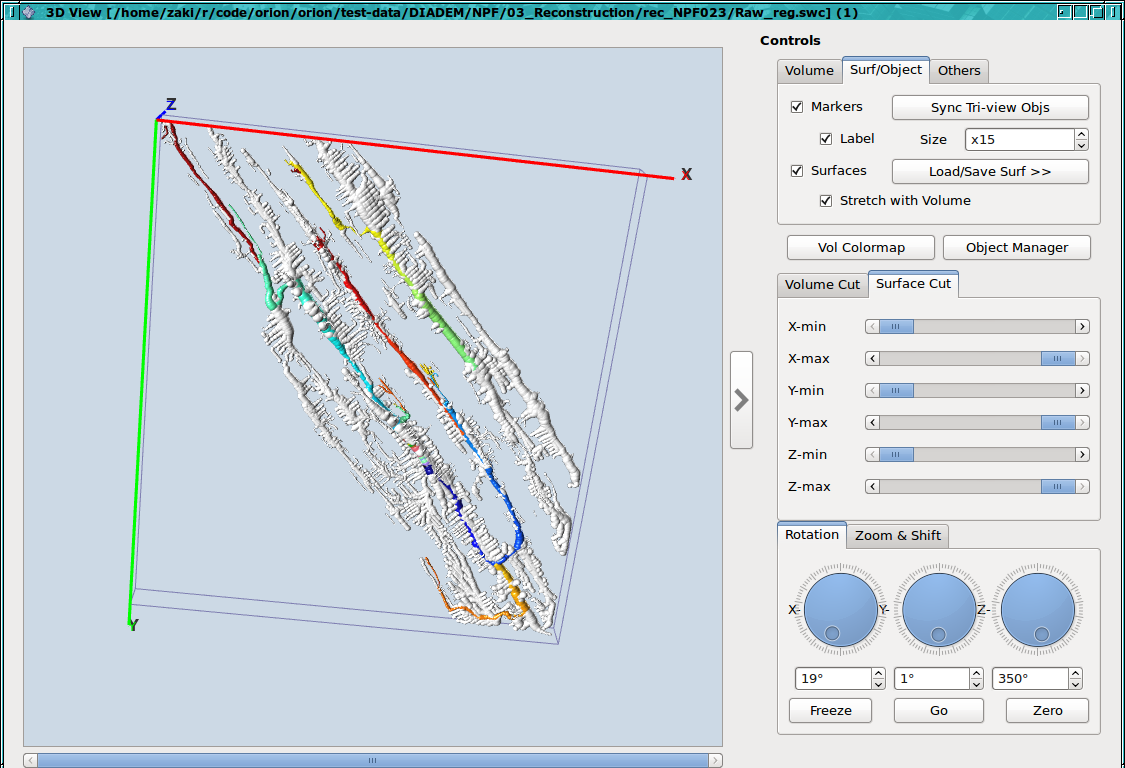
\includegraphics[height=0.5\textheight]{gfx/present/vaa3d-load-swc}
	\note{
		This is a neuron tracing loaded into Vaa3D.
	}
\end{frame}

\subsection{ORION}
\begin{frame}\frametitle{\subsecname}
	\begin{enumerate}
		\def\labelenumi{\arabic{enumi}.}
		\item Segmentation
		\item Tracing
	\end{enumerate}
\end{frame}

\begin{frame}\frametitle{ORION: Segmentation}
	Given volume \(\InputVolumeName\) and scales \(\RadiiScalesElem \in \RadiiScalesName\):
	\begin{enumerate}
		\def\labelenumi{\arabic{enumi}.}
		\item Detect training points
		\begin{enumerate}
			\def\labelenumii{\arabic{enumii}.}
			\item Create a Laplacian filter of scale
				\(\LaplacianScalesElem\): \(\LaplacianOutputVolumeElem\)
			\item Create a filter from the second
				derivatives of a Gaussian of scale
				\(\RadiiScalesElem\) to compute
				the two largest eigenvalues of the Hessian:
				\(\EigSecondElem\) and
				\(\EigThirdElem\).
			\item For each voxel, find the \(\ScaleIndex^{th}\) scale which has
				a maximum response to
				\(\LaplacianOutputVolumeElem\).
				Assign the two largest eigenvalues
				to a feature vector.
		\end{enumerate}
	\end{enumerate}
\end{frame}

\begin{frame}[fragile]
\frametitle{Feature Extraction}
 %% Mathematical commands
\resizebox{1.0\textwidth}{!}{
\begin{tikzpicture}[node distance=3cm and 1cm]
  \tikzset{
    every node/.style={font={\Large}},
    invisible/.style={opacity=0, decoration = {visibility=0}},
    transparent/.style={opacity=0.5, text opacity=0.9, decoration = {visibility=0.5}},
    visible/.style={opacity=1, font={\Large\be}, decoration = {visibility=1}},
    visible on/.style={temporal=#1{invisible}{visible}{transparent}},
    temporal/.code args={<#1>#2#3#4}{%
      \temporal<#1>{\pgfkeysalso{#2}}{\pgfkeysalso{#3}}{\pgfkeysalso{#4}
      } % \pgfkeysalso doesn't change the path
    },
  }
%% Input nodes
\node[data, label={[align=left] below:Scalar Degree of Taylor}, visible on=<1->] (dl) at (0, 12) {$d^{L}$};
\node[data, label={[align=left] below:$M = m_{0}  \times m_{1} \times m_{2} $\\ Volume of \\ intensity pixels}, visible=<1->] (Vijk) at (0,6) {$V\InputVolumeIndices$};
\node[data, label={[align=left] below:$n$-vector\\ with elements\\ representing\\ the radius to\\ segment (scale)}, visible on=<1->] (rs) at (0,0) {$r_{s}$};

%% First row nodes
\node[function, right=of Vijk, visible on=<2>] (field21) {Laplacian\\ scale\\ parameter};
\node[data, right=of field21, visible on=<3>, label={[align=left, visible on=<3>] below:$\Dim{\RadiiScalesName}-vector$}] (field22) {$\sigma^{G}_{s}$};
\node[function, right=of field22, visible on=<4>] (field23) {Laplacian\\ filter\\ (HDAF)};
\node[data, right=of field23, visible on=<5>] (field24) {$V^{L}_{s}\InputVolumeIndices$};
\node[function, right=of field24, visible on=<6>,text width=4.5cm] (field25) {$\displaystyle\argmax_{s}V^{L}_{s}\InputVolumeIndices$};

\node[data, right=of field25, visible on=<7>, label={[align=left, visible on=<7>] below:M volume of $s^{th}$\\  index elements}] (field26) {$R_{\mathrm{max}}^{L}\InputVolumeIndices$};


%% Second row nodes
\node[function, right=of rs, visible on=<8>] (field11) {Hessian\\ scale\\ parameter};
\node[data, right=of field11, visible on=<9>,  label={[align=left, visible on=<9>] below:$\Dim{\RadiiScalesName}-vector$}] (field12) {$\sigma^{G}_{s}$};
\node[function, right=of field12, visible on=<10>] (field13) {Hessian\\ filter};
\node[data, right=of field13, visible on=<11>,  label={[align=left, visible on=<11>] below:$\Dim{\RadiiScalesName}-vector$}] (field14) {$ \lambda_{s,1}\InputVolumeIndices$\\ $\lambda_{s,2}\InputVolumeIndices$\\ $\lambda_{s,3}\InputVolumeIndices$\\};
\node[function, right=of field14, visible on=<12>] (field15) {$F^{G}\InputVolumeIndices$};


%% First row connections
\path[d2f, visible on=<4>] (dl) to[in=90,out=0] (field23);
\path[d2f, visible on=<4>] (Vijk) to[in=150,out=45] (field23);
\path[d2f, visible on=<10>] (Vijk) to[in=150,out=325] (field13);
\path[d2f, visible on=<2>] (rs) to[in=225,out=15] (field21);
\path[d2f, visible on=<8>] (rs) to[in=180,out=0] (field11);

%% L1
\path[f2d, visible on=<9>] (field11) to[in=180,out=0] (field12);
\path[d2f, visible on=<10>] (field12) to[in=180,out=0] (field13);
\path[f2d, visible on=<11>] (field13) to[in=180,out=0] (field14);
\path[d2f, visible on=<12>] (field14) to[in=180,out=0] (field15);

%% L2
\path[f2d, visible on=<3>] (field21) to[in=180,out=0] (field22);
\path[d2f, visible on=<4>] (field22) to[in=180,out=0] (field23);
\path[f2d, visible on=<5>] (field23) to[in=180,out=0] (field24);
\path[d2f, visible on=<6>] (field24) to[in=180,out=0] (field25);
\path[f2d, visible on=<7>] (field25) to[in=180,out=0] (field26);

\end{tikzpicture}
}
\end{frame}


\begin{frame}
	\begin{figure}
		\centering
		\resizebox{0.9\textwidth}{!}{\begin{tikzpicture}[node distance=0.5cm]
	\tikzstyle{step} = [draw,shape=circle,scale=0.4];
	%
	\node (step_shortest_path)        at (0,0)             [draw,step] {\parbox{3cm}{\centering{}Shortest path using fast-marching}};

	\node (step_centre_pts)          [right=of step_shortest_path]    [draw,step] {\parbox{2cm}{\centering{}Centre of dendrite}};
	\node (step_radii_estimation)    [right=of step_centre_pts]       [draw,step] {\parbox{2cm}{\centering{}Radii estimation}};
	\node (step_neumorph_repr)       [below=of step_radii_estimation] [draw,step] {\parbox{3cm}{\centering{}Neuron morphology representation}};
	\node (step_post)                [left=of step_neumorph_repr]    [draw,step] {\parbox{2cm}{\centering{}Post-processing of tracing}};

	\draw [->] (step_shortest_path)    -- (step_centre_pts);
	\draw [->] (step_centre_pts)       -- (step_radii_estimation);
	\draw [->] (step_radii_estimation) -- (step_neumorph_repr);
	\draw [->] (step_neumorph_repr)    -- (step_post);
%
\end{tikzpicture}
}
		%\caption[Diagram of tracing process]{\textbf{Diagram of tracing process}}\label{fig:proc-tracing}
	\end{figure}
\end{frame}

%  - Proposed Framework - this is the most important part of your proposal.
%        Expect most questions from committee members on this. Put in all your
%        best here. Describe the entire framework before separating into work-done and
%        work-left. Do not mix framework with results. You may start with a one-slide
%        overview of the entire framework before going into details. Make sure committee
%        members will be able to understand your work. Relate to previous approaches and
%        how your is an extension or a difference. Include mathematical equations that
%        will explain your work.
%  - Explain the relevance of each equation. Understand the meaning and
%        significance of each term in the equation irrespective of whether you define
%        them in the slide or not. TIP: Rather than doing your equation twice (for your
%        PPT and Latex write-up), you may do it once in your Latex document and copy
%        into TexPoint for the PPT.
%  - Preliminary Results - if you already have some results, please show it.
%        Talk about how you propose to validate your results. Show how your
%        results compare with previous results OR how it performs in general, (e.g., in
%        how many images it succeeded or in how many it failed). A chart will be useful.
%        Any statistical comparison should indicate level of significance.
%  - Present status of the proposed framework
%        - which aspects are completed, which are in progress, and which have not yet been done at all.
%  - It is advisable to include a timeline of future indicating milestones and when you hope to achieve each.
%  - Expected Impact - mention specific application areas where you have tried or will try your proposed framework.
%        Also, explain how it can be generalized to other areas in Computer
%        Science. What is the overall benefit for the community? What is the
%        contribution to Computer Science research?

\section{Methods}

\subsection{Conversion}
\begin{frame}\frametitle{\subsecname}
	\begin{itemize}
		\item<1-> Rewrite vs. Refactor
		\item<2-> MATLAB version: \gls{orionmat}
		\item<2-> C version: \gls{orionc}
		\item<3-> Work function-by-function
	\end{itemize}
\end{frame}

\subsubsection{Conversion challenges}
\begin{frame}\frametitle{\subsubsecname}
		\begin{itemize}
			\item<1-> C is very different from MATLAB
			\item<2-> No existing tests
			\item<3-> Remove code that is MATLAB specific
		\end{itemize}
	\note{
	[\tbackground{challenges when doing a rewrite from MATLAB to native code}]
	}
\end{frame}

\begin{frame}\frametitle{Data handling}
	\begin{itemize}[<+->]
		\item Caching
		\item Subvolume
	\end{itemize}
	\note{
		\begin{itemize}
		\item
		  Original code attempts to speed up subsequent runs by saving
		  intermediate results.
		\item
		  Breaks up large volumes into small volumes
		\item
		  This is fine, but every part of the codebase uses the same data by
		  reading from files.
		\end{itemize}
	}
\end{frame}

\begin{frame}\frametitle{Coupling via cross-cutting concerns}
	\begin{figure}[tbp]
	\centering
	%% Cross cutting concerns
\usetikzlibrary{arrows,calc}
\begin{tikzpicture}[node distance=1cm, >= triangle 60]

	\tikzstyle{process} = [draw,shape=rectangle,scale=0.7]
	\tikzstyle{data} = [draw,shape=circle,style=dashed,scale=0.5]
	%
	\node (data0)        at (0,0)              [data] {data file a};
	\node (data1)        [right=of data0]      [data] {data file b};
	\coordinate (Middle) at ($(data0)!0.5!(data1)$);

	\node (proc0)        [below left=of data0] [process] {Module 0};
	\node (proc1)        [below=of Middle] [process] {Module 1};
	\node (proc2)        [right=of proc1] [process] {Module 2};

	%\node (data_centreline) [right=of proc_trace] [data] {$\mathrm{Centerline}$};

	\draw [<-] (data0)   --  (proc0);
	\draw [<-] (data1)   --  (proc0);

	\draw [->] (data0)   --  (proc1);
	\draw [->] (data1)   --  (proc1);

	\draw [->] (data0)   --  (proc2);
	\draw [->] (data1)   --  (proc2);
%
\end{tikzpicture}


	\caption{\textbf{Files accessed by multiple modules}
	}\label{fig:ccc}
	\end{figure}

	\note{
		\begin{itemize}
			\item
				As soon as you make changes in one, you have to change the others.
			\item
				Imagine changing the file name
			\item
				Writes to the file-system, so it will needs file locking if run in
				parallel
		\end{itemize}
	}
\end{frame}

\begin{frame}\frametitle{Reducing coupling via indirection}
	\begin{figure}[tbp]
	\centering
	%% Cross cutting concerns solved with a DAO
\usetikzlibrary{arrows}
\begin{tikzpicture}[node distance=1cm, >= triangle 60]

	\tikzstyle{process} = [draw,shape=rectangle,scale=0.7]
	\tikzstyle{data} = [draw,shape=circle,style=dashed,scale=0.5]
	\tikzstyle{object} = [draw,shape=circle,style=solid,scale=0.5]
	%
	\node (dao)        at (0,0)      [object] {data access object};

	\node (data0)        [above left=of dao]              [data] {data file a};
	\node (data1)        [above right=of dao]      [data] {data file b};

	\node (proc0)        [below left=of dao] [process] {Module 0};
	\node (proc1)        [below=of dao] [process] {Module 1};
	\node (proc2)        [below right=of dao] [process] {Module 2};

	%\node (data_centreline) [right=of proc_trace] [data] {$\mathrm{Centerline}$};

	\draw [<->] (dao)   --  (data0);
	\draw [<->] (dao)   --  (data1);

	\draw [<-] (dao)   --  (proc0);
	\draw [<-] (dao)   --  (proc0);

	\draw [->] (dao)   --  (proc1);
	\draw [->] (dao)   --  (proc1);

	\draw [->] (dao)   --  (proc2);
	\draw [->] (dao)   --  (proc2);
%
\end{tikzpicture}


	\caption{\textbf{Using a data access object to reduce coupling}
	}\label{fig:ccc-dao}
	\end{figure}

	\note{
		\begin{itemize}
			\item Any problem in CS can be solved by adding another layer of indirection.
			\item Possible solution: Add another layer of indirection via a Data Access Object (DAO)
			\item Reduces coupling between business logic and persistence logic
			\item Persistence logic can be swapped out
		\end{itemize}
	}
\end{frame}

\subsection{Roads not taken}
\begin{frame}<1>[label=frost]\frametitle{Roads not taken}
\begin{itemize}
	\item<1> MATLAB Engine API
	\item<2> MATLAB Compiler Runtime
\note{
}
% TODO describe MATLAB Engine API and MATLAB Compiler Runtime
\end{itemize}
\end{frame}

\subsubsection{Call graph}
\begin{frame}\frametitle{\subsubsecname}
	\begin{tabular}{p{0.4\textwidth}c}
		\begin{minipage}{\linewidth}
			\begin{itemize}
				\item<1-> Already existing architecture
				\item<2-> Create a graph of function calls
				\item<3-> Provides an order to work in
			\end{itemize}
		\end{minipage}
		&
		\begin{minipage}{\linewidth}
		%\vertcenterimage{\includegraphics[height=0.3\textheight]{gfx-out/matlab-call-graph/segmentation.tex}}
		\resizebox{0.6\linewidth}{!}{\begin{tikzpicture}[node distance=0.5cm]
	\tikzstyle{step} = [draw,shape=circle,scale=0.4];
	%
	\node (step_bg_train)        at (0,0)             [draw,step] {\parbox{3cm}{\centering{}Obtain background training data}};

	\node (step_feat)        [right=of step_bg_train] [draw,step] {\parbox{2cm}{\centering{}Obtain vessellness features}};
	\node (step_discrim)     [right=of step_feat]     [draw,step] {\parbox{2cm}{\centering{}Learn discriminant function}};
	\node (step_thresh)      [below=of step_discrim]  [draw,step] {\parbox{2cm}{\centering{}Threshold}};
	\node (step_post)        [left=of step_thresh]    [draw,step] {\parbox{2cm}{\centering{}Post-processing}};

	\draw [->] (step_bg_train) -- (step_feat);
	\draw [->] (step_feat) -- (step_discrim);
	\draw [->] (step_discrim) -- (step_thresh);
	\draw [->] (step_thresh) -- (step_post);
%
\end{tikzpicture}
}
		\end{minipage}
	\end{tabular}
	\note{
	[\tbackground{analysis of existing codebase; how this informs the new
	implementation; why use the call graph instead of
	attempting to either do a clean room implementation (i.e.,
	by only reading papers) or creating a new architecture
	from scratch}]
	}
\end{frame}

\subsubsection{Directory structure}
\begin{frame}\frametitle{\subsubsecname}
	\begin{itemize}
		\item<1-> \computertext{lib/container}: container data structures (e.g., resizable arrays)
		\item<2-> \computertext{lib/ndarray}: n-dimensional array and volume processing code (e.g., FFT)
		\item<3-> \computertext{lib/numeric}: numeric helper functions (e.g., polynomial calculation)
		\item<4-> \computertext{lib/simple-log}: logging code
	\end{itemize}
	\note{
	[ plan for the directory structure (where does each file
	go) ]
	}
\end{frame}

\begin{frame}\frametitle{\subsubsecname}
	\begin{itemize}
		\item<1-> \computertext{lib/kitchen-sink}: implementation of functions that match \gls{orionmat} code
		\item<2-> \computertext{lib/vaa3d-plugin}: code to integrate with Vaa3D
		\item<3-> \computertext{lib/t}: tests for all the above
	\end{itemize}
\end{frame}

\subsection{Integration}
\begin{frame}\frametitle{\subsecname}
	\begin{itemize}
		\item BigNeuron requires working with Vaa3D
		\item Use a standard API for all algorithms
	\end{itemize}
	\note{
	[\tbackground{description of Vaa3D}]
	}
\end{frame}

\subsubsection{Vaa3D integration}
\begin{frame}\frametitle{\subsubsecname}
	\centering
	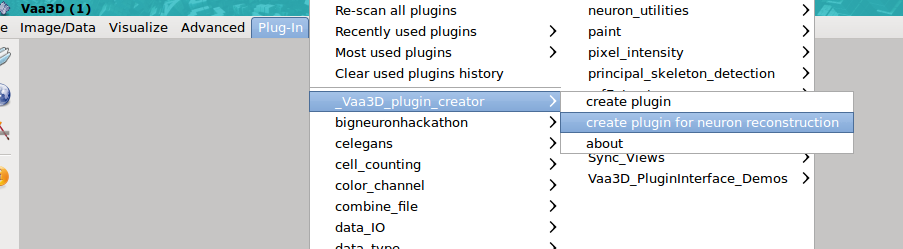
\includegraphics[height=0.3\textheight]{gfx/present/vaa3d-create-neuron-rec-plugin}
	\note{
		The idea behind contributing an algorithm to
		BigNeuron is to create a plugin that will take
		data in a standarised form and give back a
		reconstruction in a standardised form.
	}
\end{frame}

\subsection{Testing and Reproducibility}
\begin{frame}\frametitle{\subsecname}
	\begin{itemize}
		\item<1-> Write simple tests: simple to read, simple to verify
		\item<2-> Sanity checking
		\item<3-> Are dependencies working as expected?
		\item<4-> Tests can be run by others
	\end{itemize}
	\note{
	[\tmetrics{why testing is important}]
	}
\end{frame}

\subsubsection{Testing procedure}
\begin{frame}\frametitle{\subsubsecname}
	\begin{itemize}
		\item<1-> Analytic solutions
		\item<2-> Property testing
		\item<3-> Floating point
		\item<4-> Integration: test whole pipeline with data
	\end{itemize}
	\note{
	[
		testing procedure (TAP harness, floating point
		issues); integration testing with Vaa3D
	]
	}
\end{frame}

\section{Results}

\subsection{Results for Conversion}

\subsubsection{Qualitative results}
\begin{frame}\frametitle{\subsecname}
	% TODO
	\vertcenterimage{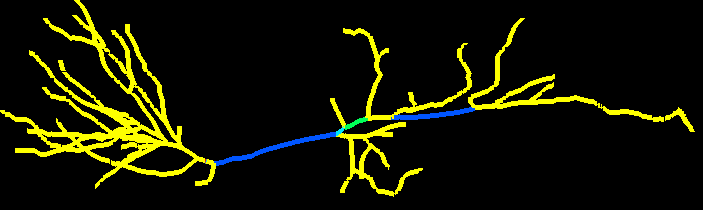
\includegraphics[width=0.8\textwidth]{gfx/present/neuron-trace}}
	\note{
	[
		\tmetrics{%
			run code on DIADEM data and show the
			visualization
		}
	]
	}
\end{frame}

%\subsubsection{Quantitative Tracing-based comparison}
%\begin{frame}\frametitle{\subsecname}
	%% TODO
	%[ get all intermediate results from MATLAB code and
	%compare to the native code (floating point for volumes,
	%tree metrics for the tracings); run on DIADEM data]
%\end{frame}

\subsection{Results for Integration}
\begin{frame}\frametitle{\subsecname}
	\begin{itemize}
		\item Load TIFF stack into Vaa3D
		\item Run plugin code
	\end{itemize}
	%[\tmetrics{a demonstration video; visual results and metrics from using
			%Vaa3D with neuron data from DIADEM; demonstration of any further analysis
	%that can be done in Vaa3D}]
\end{frame}

\begin{frame}% TODO title
\begin{figure}[H]
\centering
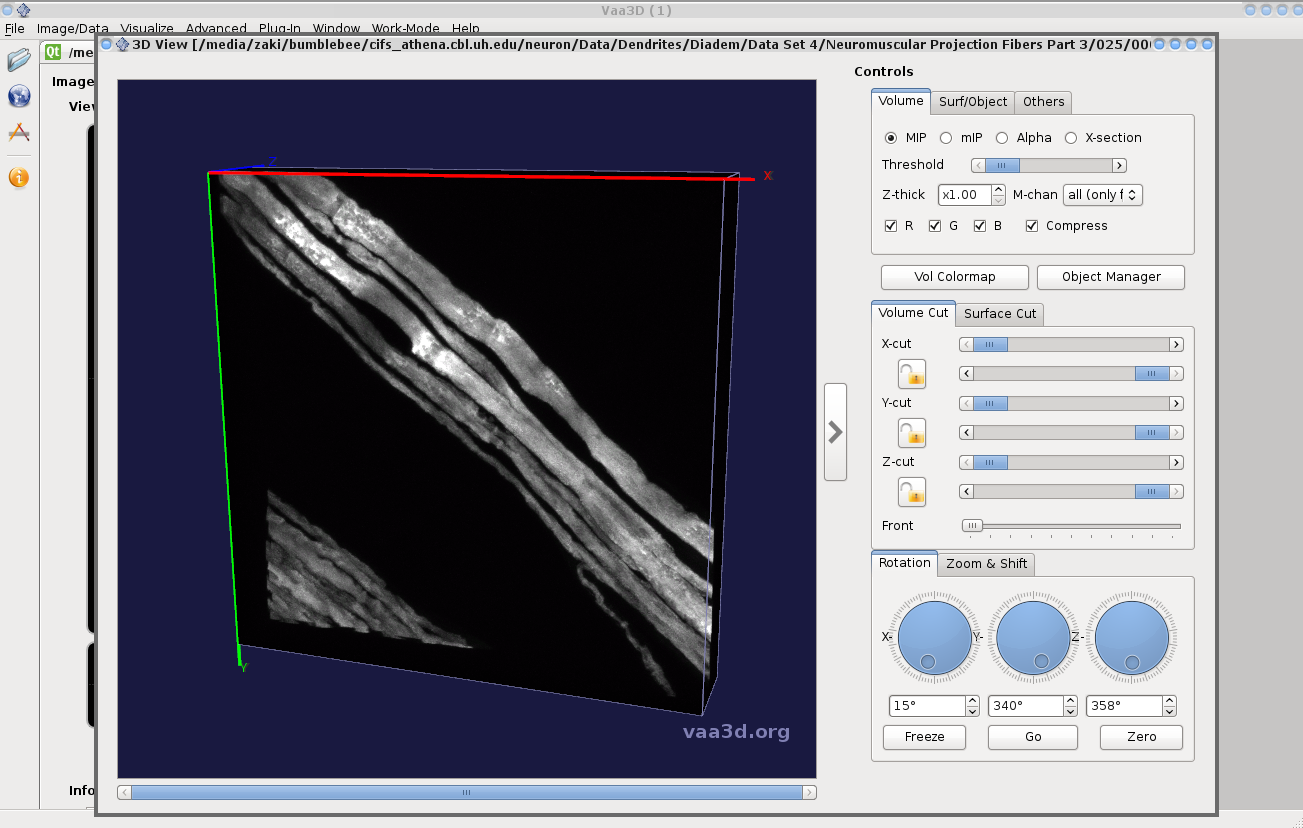
\includegraphics[width=0.8\textwidth]{gfx/vaa3d_DIADEM-NPF-3-025_3D-view}
\caption{Vaa3D: Visualization of NPF025 TIFF stack}
\end{figure}
\end{frame}

\begin{frame}% TODO title
\begin{figure}[H]
\centering
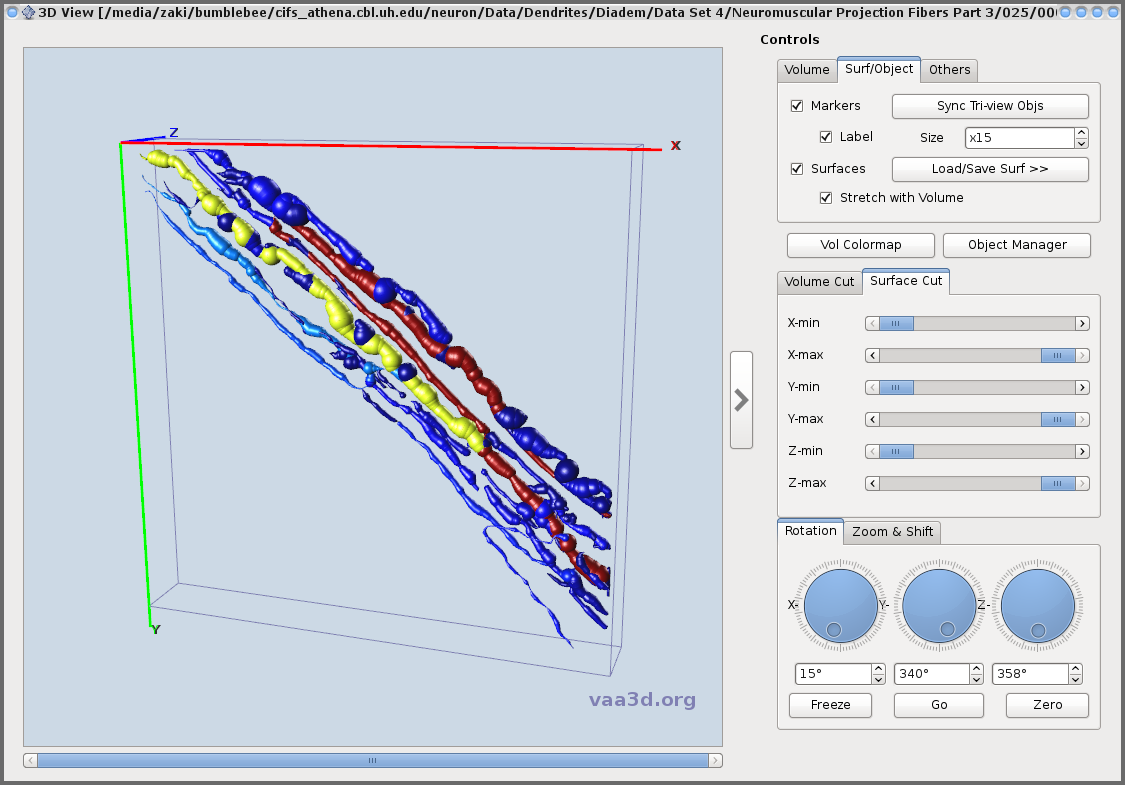
\includegraphics[width=0.8\textwidth]{gfx/vaa3d_DIADEM-NPF-3-025_APP2-tracing-3D-view}
\caption{Vaa3D: Tracing of NPF025 using Vaa3D plugin}
\end{figure}
\end{frame}

\subsection{Results for Testing and Reproducibility}

\subsubsection{Overview of tests}
\begin{frame}\frametitle{\subsubsecname}
	\begin{itemize}
		\item<1-> Numeric tests: does factorial work?
		\item<2-> I/O tests: can data be read from disk properly?
		\item<3-> Library integration: does FFT library work?
		\item<4-> Current code coverage by tests: 76.29\%.
	\end{itemize}
	\note{
	[
		overview of tests written (grouped by similarity);
		list of bugs fixed in ORION due to testing;
		code coverage; list of dead code found
	]
	}
\end{frame}

\begin{frame}\frametitle{\subsubsecname}
	\begin{itemize}
		\item<1-> Tests fix bugs and anticipate change
		\item<2-> Is the filter really isotropic?
		\item<3-> ITK Hessian filter and volume spacing changes
		\item<3-> Differences in compilers
	\end{itemize}
\end{frame}

\subsubsection{Dependency tracking}
\begin{frame}\frametitle{\subsubsecname}
	\note{
	[dependency tracking by keeping version controlled copies
		of dependencies; screenshots of all repos of deps used under the CBL-ORION
	namespace on GitHub
	]
	}
		\begin{figure}[tbp]
			\centering
			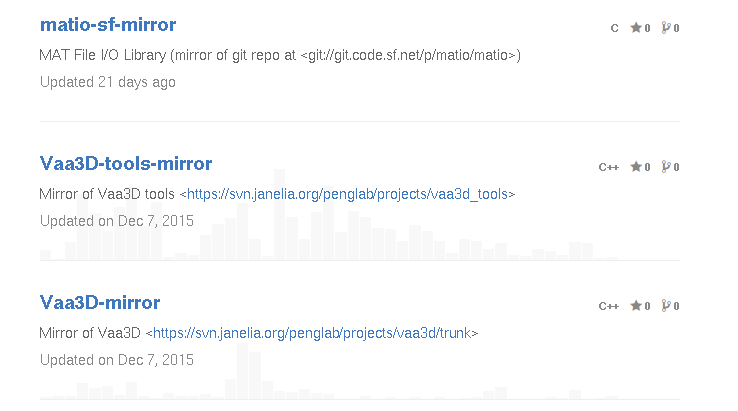
\includegraphics[width=1.0\textwidth]{gfx/gh-dep_0}
		\end{figure}
\end{frame}

\begin{frame}\frametitle{\subsubsecname}
	\begin{figure}[tbp]
		\centering
		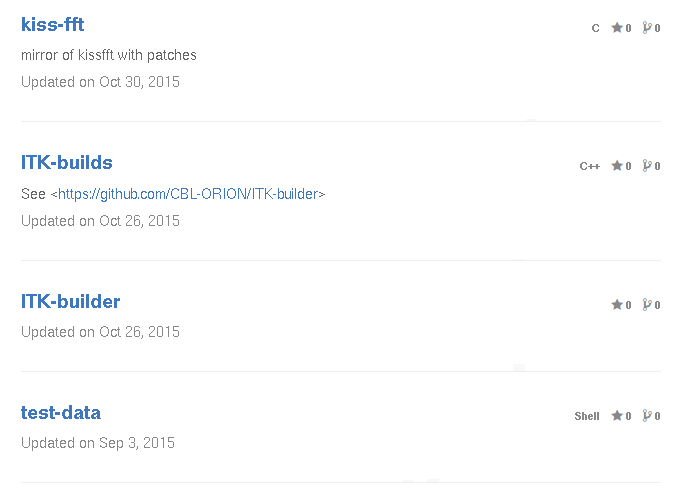
\includegraphics[width=0.9\textwidth]{gfx/gh-dep_1}
	\end{figure}
\end{frame}

\subsubsection{Documentation}
\begin{frame}\frametitle{\subsubsecname}
	\note{
	[ screenshot of documentation ]
	}
		\begin{figure}[tbp]
			\centering
			% <https://github.com/CBL-ORION/orion/wiki>
			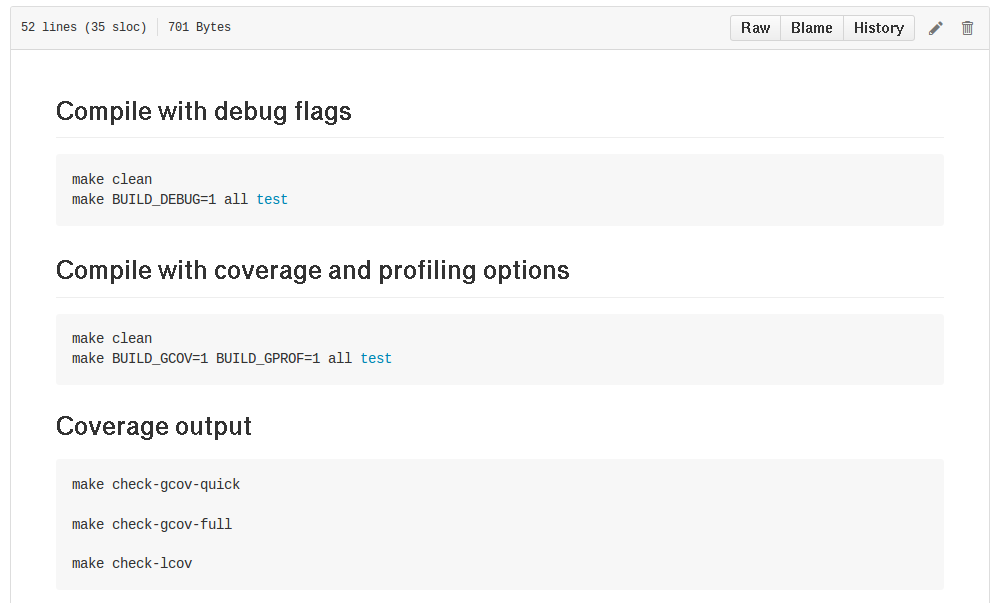
\includegraphics[width=1.0\textwidth]{gfx/doc-dev}
			\caption{\textbf{Documentation website}
			}\label{fig:doc-wiki}
		\end{figure}
\end{frame}


\subsubsection{Continuous integration}
%\note{
%[
	%{screenshots of continuous integration}
%]
%}
\begin{frame}\frametitle{\subsecname} \centering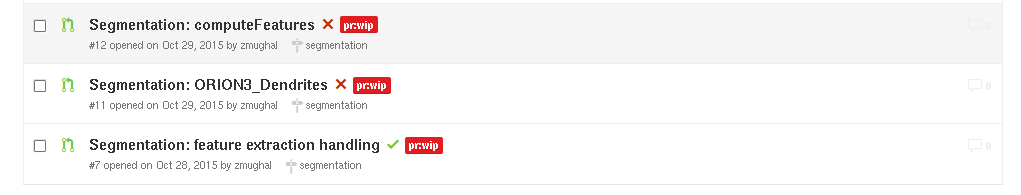
\includegraphics[width=1.0\textwidth]{gfx/ci-0} \end{frame}
\begin{frame}\frametitle{\subsecname} \centering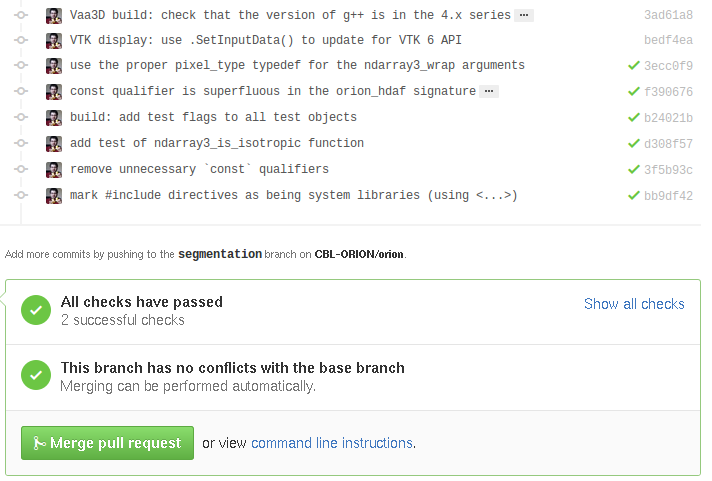
\includegraphics[width=1.0\textwidth]{gfx/ci-1} \end{frame}
\begin{frame}\frametitle{\subsecname} \centering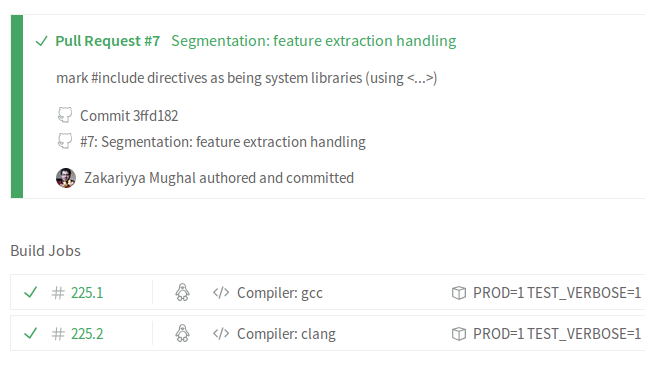
\includegraphics[width=1.0\textwidth]{gfx/ci-2} \end{frame}
\begin{frame}\frametitle{\subsecname} \centering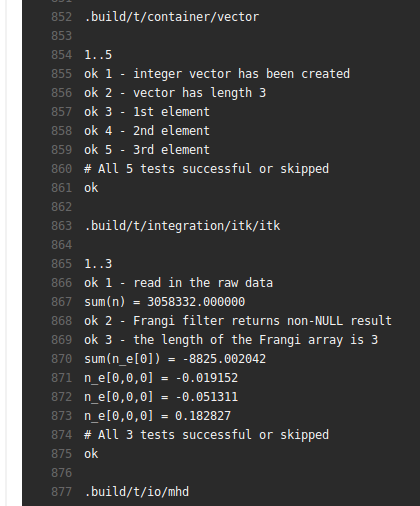
\includegraphics[height=0.65\textwidth]{gfx/ci-3} \end{frame}

\begin{frame}\frametitle{Estimating error in stages}
\begin{figure}
	  % Cases
	  \definecolor{inputcol}{RGB}{0,0,0}
	  \definecolor{lgray}{RGB}{192,192,192}
	  \definecolor{ngray}{RGB}{160,160,160}
	  \definecolor{dgray}{RGB}{128,128,128}

	  \definecolor{tcol}{RGB}{255,255,255}
	  % Cases
	  \definecolor{lblue}{RGB}{102,102,255}
	  \definecolor{nblue}{RGB}{51,51,255}
	  \definecolor{dblue}{RGB}{0,0,255}
	\resizebox{0.8\linewidth}{!}{%\documentclass[tikz, border=10pt]{standalone}
\tikzset{
    vertex/.style = {
        circle,
        fill            = black,
        outer sep = 2pt,
        inner sep = 1pt,
    }
}

%\begin{document}

\newcommand{\myfun}[2] {$fun^{#1}_{#2}$}
  
\begin{tikzpicture}
  % Cases
  \definecolor{lgray}{RGB}{192,192,192}
  \definecolor{ngray}{RGB}{160,160,160}
  \definecolor{dgray}{RGB}{128,128,128}
  % Cases
  \definecolor{lblue}{RGB}{102,102,255}
  \definecolor{nblue}{RGB}{51,51,255}
  \definecolor{dblue}{RGB}{0,0,255}
% Input node
\node[draw,fill=black,text=white,rotate=90] (Input) at (2,2) {Input};  
  
% Matlab nodes
\node[draw,fill=lgray,text=white] (funM1) at ( 4,0) {\myfun{M}{1}};
\node[draw,fill=lgray,text=white] (funM2) at ( 7,0) {\myfun{M}{2}};
\node[draw,fill=lgray,text=white] (funM3) at (10,0) {\myfun{M}{3}};
\node[draw,fill=lgray,text=white] (funM4) at (13,0) {\myfun{M}{4}};
\node[draw,fill=lgray,text=white] (funM5) at (16,0) {\myfun{M}{5}};

% MC nodes
\node[draw,fill=ngray,text=white] (funMC1) at ( 4,2) {\myfun{M-C}{1}};
\node[draw,fill=ngray,text=white] (funMC2) at ( 7,2) {\myfun{M-C}{2}};
\node[draw,fill=ngray,text=white] (funMC3) at (10,2) {\myfun{M-C}{3}};
\node[draw,fill=ngray,text=white] (funMC4) at (13,2) {\myfun{M-C}{4}};
\node[draw,fill=ngray,text=white] (funMC5) at (16,2) {\myfun{M-C}{5}};

% C nodes
\node[draw,fill=dgray,text=white] (funC1) at ( 4,4) {\myfun{C}{1}};
\node[draw,fill=dgray,text=white] (funC2) at ( 7,4) {\myfun{C}{2}};
\node[draw,fill=dgray,text=white] (funC3) at (10,4) {\myfun{C}{3}};
\node[draw,fill=dgray,text=white] (funC4) at (13,4) {\myfun{C}{4}};
\node[draw,fill=dgray,text=white] (funC5) at (16,4) {\myfun{C}{5}};


% Initial data conection
\draw[->,draw=dblue] (Input) to[in=180,out=0] (funC1);
\draw[->,draw=nblue] (Input) to[in=180,out=0] (funMC1);
\draw[->,draw=lblue] (Input) to[in=180,out=0] (funM1);

% C
\draw[->,draw=dblue] (funC1) to[in=180,out=0] (funC2);
\draw[->,draw=dblue] (funC2) to[in=180,out=0] (funC3);
\draw[->,draw=dblue] (funC3) to[in=180,out=0] (funC4);
\draw[->,draw=dblue] (funC4) to[in=180,out=0] (funC5);

% MC
\draw[->,draw=nblue] (funM1) to[in=180,out=0] (funMC2);
\draw[->,draw=nblue] (funM2) to[in=180,out=0] (funMC3);
\draw[->,draw=nblue] (funM3) to[in=180,out=0] (funMC4);
\draw[->,draw=nblue] (funM4) to[in=180,out=0] (funMC5);

% M
\draw[->,draw=lblue] (funM1) to[in=180,out=0] (funM2);
\draw[->,draw=lblue] (funM2) to[in=180,out=0] (funM3);
\draw[->,draw=lblue] (funM3) to[in=180,out=0] (funM4);
\draw[->,draw=lblue] (funM4) to[in=180,out=0] (funM5);


\end{tikzpicture}

\begin{tikzpicture}
  % Dialectics
  \node[draw] (Thesis) at (0,0) {Thesis};
  \node[draw,fill=black,text=white] (Antithesis) at (2.3,0) {Antithesis};
  \node[draw,fill=gray,text=white] (Synthesis) at (1,2) {Synthesis};
  
  \draw node[vertex] (Joint) at (1,0) {};
  
  \draw[-,draw=blue] (Thesis) to (Joint);
  \draw[-,draw=blue] (Antithesis) to (Joint);
  \draw[->,draw=blue] (Joint) to (Synthesis);
  \draw[->,draw=blue] (Synthesis) to[in=180,out=180] (Thesis);
  
  \node at (1.0, -1.0) {\textit{a) Dialectics}};
  
  % Opposition
  \node[draw] (ArgumentA) at (5,0) {Argument};
  \node[draw,fill=black,text=white] (ArgumentB) at (7.5,0) {Opposition};
  
  \draw[->,draw=blue] (ArgumentA) to (ArgumentB);
  
  \node at (6., -1.0) {\textit{b) Opposition}};
  
  % Innovation
  \node[draw] (ArgumentA) at (10.1,0) {Argument};
  \node[draw,fill=black,text=white] (ArgumentB) at (13,0) {Opposition};
  \node[draw,fill=yellow] (ArgumentC) at (12,2) {Innovation};
  
  \draw node[vertex] (Joint) at (11.5,0) {};
  
  \draw[-] (ArgumentA) to (Joint);
  \draw[-] (ArgumentB) to (Joint);
  \draw[->,draw=blue] (Joint) to (ArgumentC);
  
  \node at (11.5, -1.0) {\textit{c) Innovation}};
\end{tikzpicture}
%\end{document}}
	\caption{Full pipeline}
\end{figure}
\end{frame}

\begin{frame}\frametitle{Estimating error in stages}
	\begin{itemize}
	\item<1-> Set breakpoints at every function start and end
	\item<2-> Run the MATLAB code
	\item<3-> Save the state of the input and output data at
		each breakpoint with stack frame ID
	\end{itemize}
\end{frame}

\begin{frame}\frametitle{Estimating error in stages}
	\begin{itemize}
		\item<1-> Load the MATLAB data
		\item<2-> Convert MATLAB to C data structures
		\item<3-> Compare the results using an appropriate method
	\end{itemize}
\end{frame}

\begin{frame}\frametitle{Estimating error for Makefilter}
	\centering
	%	\begin{tabular}{lcccc}
		\toprule
                  \be{}Setup                              & \be{}one                    & \be{}two                    & \be{}three                  & \be{}four                   \\%\hline
		\midrule
                  \be\gls{orionmat}                     & \cellcolor{langM} x(1) & \cellcolor{langM} x(2) & \cellcolor{langM} x(3) & \cellcolor{langM} x(4) \\%\hline
                  \be\gls{orionc}                       & \cellcolor{langC} x[0] & \cellcolor{langC} x[1] & \cellcolor{langC} x[2] & \cellcolor{langC} x[3] \\%\hline
                  \be\gls{orionmattoc}                  & \cellcolor{langCM} 4   & \cellcolor{langCM} 3   & \cellcolor{langCM} 2   & \cellcolor{langCM} 1   \\%\hline
                  \be\gls{orionmat} - \gls{orionc}      & \cellcolor{diffone} 4  & \cellcolor{diffone} 3  & \cellcolor{diffone} 2  & \cellcolor{diffone} 1  \\%\hline
                  \be\gls{orionmat} - \gls{orionmattoc} & \cellcolor{difftwo} 4  & \cellcolor{difftwo} 3  & \cellcolor{difftwo} 2  & \cellcolor{difftwo} 1  \\%\hline
		\bottomrule
        \end{tabular}

	\begin{tabular}{cc}
		\toprule
                  \be{}Stack ID                              & \be{} histogram intersection \\
		\midrule
			1 & 0.999973665203964 \\
			2 & 0.999967508148729 \\
			3 & 0.999978416844418 \\
			4 & 0.999982131154914 \\
			5 & 0.999959276433577 \\
		\bottomrule
        \end{tabular}
\end{frame}

\section{Conclusion}
%  - Conclusion slide could be catchy, something they will remember.
%        Maybe an animation, video, or terse statement that summarizes it all.
\begin{frame}\frametitle{\secname}
	\begin{itemize}
		\item<1-> Project set up for future work
		\item<2-> Automatic testing for every change
		\item<3-> Can be packaged for Vaa3D, NeuroDebian
	\end{itemize}
	\note{
	[
		mention future work (e.g., NeuroDebian)
	]
	}
\end{frame}

\begin{frame}\frametitle{\secname}
	\centering\Huge Questions?
\end{frame}

%  - Publications - you should list your publications or mention them in relevant sections of the presentation.


\end{document}
